\chapter{Funktionentheorie}
\label{\detokenize{complexanalysis/complexanalysis:funktionentheorie}}\label{\detokenize{complexanalysis/complexanalysis::doc}}
\par
Im letzten Kapitel der Vorlesung widmen wir uns der \emph{Funktionentheorie}.
Diese befasst sich hauptsächlich mit der Theorie differenzierbarer komplexer Funktionen.
Da viele Konzepte der reellen Analysis verwendet werden, wird dieses Gebiet auch häufig \textbf{komplexe Analysis} genannt.

\par
Die Grundlagen des Körpers der komplexen Zahlen wurden bereits in \cite{Ten21} behandelt. Als Referenz empfehlen wir hier wiederum das Skript von Prof.Dr.Hermann Schulz Baldes \cite{SB18} aber auch das Skript zur Funktionentheorie von Prof.Dr.Karl Hermann Neeb \cite{Nee17}. Teile des im Folgenden präsentierten Stoffs basieren auf diesen Referenzen.


\section{Die Komplexen Zahlen}
\label{\detokenize{complexanalysis/complexnumbers:die-komplexen-zahlen}}\label{\detokenize{complexanalysis/complexnumbers::doc}}
\par
Wir werden hier zunächst die wichtigen Grundlagen der komplexen Zahlen wiederholen.
Die komplexen Zahlen werden eingeführt als das Tupel
\begin{align*}
\C := (\R^2,+,\cdot)
\end{align*}
\par
zusammen mit den Operationen
\begin{align*}
(x_1,y_1) + (x_2,y_2) &:= (x_1 + x_2, y_1+y_2),\\
(x_1,y_1) \cdot (x_2,y_2) &:= (x_1\cdot x_2 - y_1\cdot y_2, y_1\cdot x_2 + x_1\cdot y_2).
\end{align*}
\par
Diese Struktur bildet einen \textbf{Körper} mit dem Einselement \(1:=(1,0)\). Das Element \(i:=(0,1)\) heißt \textbf{imaginäre Einheit} und erfüllt die Gleichung
\begin{align*}
i^2 = (0,1)\cdot(0,1) = -(1,0) = -1.
\end{align*}
\par
Als reeller Vektorraum hat \(\C\) die kanonische Basis \(\{(1,0),(0,1)\}=\{1,i\}\) weshalb wir jedes Element darstellen können über
\begin{align*}
(x,y) = x + iy.
\end{align*}
\par
Für eine komplexe Zahl \(z=x+ iy\in\C\) definieren wir
\begin{enumerate}

\item {} 
\par
\(\Re(z):= x\) den \textbf{Realteil},

\item {} 
\par
\(\Im(z):=y\) den \textbf{Imaginärteil},

\item {} 
\par
\(\overline{z}:= x-iy\) die \textbf{komplexe Konjugation},

\item {} 
\par
\(\abs{z} = \sqrt{z\overline{z}} = \sqrt{x^2+y^2}\) den \textbf{Betrag}.

\end{enumerate}

\par
Für den Betrag komplexer Zahlen gelten die bekannten Rechenregeln
\begin{align*}
\abs{0}&=0,\\
\abs{z\cdot w} &= \abs{z}\cdot \abs{w},\\
\abs{z+w}&\leq\abs{z}+\abs{w},
\end{align*}
\par
für zwei komplexe Zahlen \(z,w\in\C\)

\par
Insbesondere induziert der Betrag die Metrik
\begin{align*}
d(z,w):= \abs{z-w}
\end{align*}
\par
und damit auch eine Topologie sowie die Begriffe Konvergenz und Stetigkeit einer Funktion \(f:\C\to\C\).

\par
Weiterhin lassen sich komplexe Zahlen auch in \textbf{Polarkoordinaten} darstellen, d.h., für jedes \(z\in\C\) existiert ein eindeutig bestimmter Winkel \(\varphi\in [0,2\pi]\), s.d.
\begin{align*}
z = r(\cos(\varphi) + i\sin(\varphi))
\end{align*}
\par
wobei \(r=\abs{z}\). In diesem Kontext ist auch die \textbf{Eulersche Formel} relevant,
\begin{align}\label{equation:complexanalysis/complexnumbers:eq:euler}
\exp(i\varphi) = \cos(\varphi) + i\sin(\varphi)
\end{align}
\par
für \(\varphi\in [0,2\pi]\).


\section{Holomorphe Funktionen}
\label{\detokenize{complexanalysis/cauchyriemann:holomorphe-funktionen}}\label{\detokenize{complexanalysis/cauchyriemann::doc}}
\par
Wir betrachten im Folgenden komplexe Funktionen \(f:\C\to\C\). Der Begriff der Stetigkeit wird durch die Metrik induziert. Das Konzept der Differenzierbarkeit führt auf den zentralen Begriff der Funktionentheorie, sogenannte \emph{holomorphen Funktionen}.
\begin{definition}{(Holomorphe Funktion)}{complexanalysis/cauchyriemann:def:holomorph}



\par
Sei \(U \subset \C\) eine offene Teilmenge, eine Funktion \(f:U\to\C\) heißt \textbf{komplex differenzierbar} in \(p\in\C\), falls der Grenzwert
\begin{align*}
f'(p) = \lim_{h\rightarrow 0} \frac{f(p+h) - f(p)}{h}
\end{align*}
\par
existiert. Ist \(f\) komplex differenzierbar für alle \(p\in U\) so nennen wir \(f\) \textbf{holomorph}.
\end{definition}
\begin{remark}{}{complexanalysis/cauchyriemann:remark-1}



\par
Beachte, dass im obigen Grenzwert \(h\in\C\) gilt, der Limes existiert also, falls für eine beliebige Folge \(h_k\in\C,k\in\N\) mit \(\abs{h_k}\to 0\) gilt, dass
\begin{align*}
\lim_{k\to\infty} \frac{f(p+h_k) - f(p)}{h_k} = f'(p).
\end{align*}
\par
Dies ist äquivalent dazu, dass für eine beliebige Folge \(z_k\in\C,k\in\N\) mit \(\abs{z_k-p}\to 0\) gilt, dass
\begin{align*}
\lim_{k\to\infty} \frac{f(z_k) - f(p)}{z_k - p} = f'(p).
\end{align*}\end{remark}


\subsection{Eigenschaften holomorpher Funktionen}
\label{\detokenize{complexanalysis/cauchyriemann:eigenschaften-holomorpher-funktionen}}
\par
Eine sehr nützliche Eigenschaft komplex differenzierbarer Funktionen liefert das folgende Lemma.
\begin{lemma}{}{complexanalysis/cauchyriemann:lem:splitholo}



\par
Sei \(U \subset \C\) eine offene Teilmenge, die Funktion \(f:U\to\C\) ist genau dann komplex differenzierbar in \(p\in U\), falls eine in \(p\) stetige Funktion \(h:U\to\C\) existiert, s.d.
\begin{align*}
f(z) = f(p) + h(z)\cdot (z-p)\quad\forall z\in U.
\end{align*}
\par
Weiterhin gilt in diesem Fall \(h(p) = f^\prime(p)\).
\end{lemma}

\begin{proof}
 Es sei \(f\) komplex differenzierbar in \(p\), dann definieren wir die Funktion
\begin{align*}
h(z):=
\begin{cases}
\frac{f(z) - f(p)}{z-p}\text{ falls }z\neq p\\
f^\prime(p)\text{ sonst.}
\end{cases}
\end{align*}
\par
Da \(f\) komplex differenzierbar in \(p\) ist existiert der Grenzwert
\begin{align*}
\lim_{z\to p} \frac{f(z) - f(p)}{z-p}
\end{align*}
\par
und ist gleich \(f^\prime(p)\) und daher ist \(h\) stetig in \(p\). Weiterhin gilt
\begin{align*}
h(z)\cdot (z-p) = f(z) - f(p)\quad\forall z\in U
\end{align*}
\par
und daher die Behauptung.

\par
Für die andere Richtung sei \(h\) eine in \(p\) stetige Funktion s.d.
\begin{align*}
f(z) = f(p) + h(z)\cdot (z-p)\quad\forall z\in U.
\end{align*}
\par
Dann gilt
\begin{align*}
\lim_{z\to p} \frac{f(z) - f(p)}{z-p} = \lim_{z\to p} h(z) = h(p)
\end{align*}
\par
wobei der Grenzwert existiert, da \(h\) stetig in \(p\) ist. Somit ist \(f\) komplex differenzierbar in \(p\).
\end{proof}

\par
Mithilfe des obigen Lemmas können wir sofort folgern, dass holomorphe Funktionen stetig sind.
\begin{lemma}{}{complexanalysis/cauchyriemann:lemma-3}



\par
Es sei \(U\subset\C\) offen und \(f:U\to\C\) sei komplex differenzierbar in \(p\in U\), dann folgt \(f\) ist stetig in \(p\).
\end{lemma}

\begin{proof}
 Die Funktion \(f\) sei komplex differenzierbar in \(p\), dann existiert nach \cref{complexanalysis/cauchyriemann:lem:splitholo} eine in \(p\) stetige Funktion \(h\), s.d.,
\begin{align*}
f(z) = f(p) + h(z)\cdot(z-p)\quad \forall z\in U.
\end{align*}
\par
Die Polynome \(z\mapsto f(p), z\mapsto (z-p)\) sind jeweils stetig in \(p\), Addition und Multiplikation stetiger Funktionen erhält Stetigkeit und somit ist \(f\) stetig in \(p\).
\end{proof}

\par
Wir betrachten nun noch Ableitungsregeln, welche versichern, dass wir für die komplexe Ableitung die gewohnten Rechenregeln benutzten dürfen.
\begin{lemma}{(Komplexe Ableitungsregeln)}{complexanalysis/cauchyriemann:lemma-4}



\par
Es sei \(U\subset\C\) offen und \(f,g:U\to\C\) zwei holomorphe Funktionen, dann gilt
\begin{itemize}
\item {} 
\par
\(f+g\) ist holomorph, mit \((f+g)^\prime = f^\prime + g^\prime\),

\item {} 
\par
\(f\cdot g\) ist holomorph, mit \((f\cdot g)^\prime = f^\prime g+ f g^\prime\).

\end{itemize}

\par
Weiterhin seien \(f:U\to V, g:V\to C\) zwei holomorphe Funktionen mit \(V\subset\C\) offen, dann gilt
\begin{itemize}
\item {} 
\par
\(g\circ f\) ist holomorph mit \((g\circ f)^\prime = (g^\prime \circ f)\, f^\prime\).

\end{itemize}

\par
Zusätzlich gilt
\begin{itemize}
\item {} 
\par
\(\frac{1}{f}: U\setminus f^{-1}(0)\to \C\) ist holomorph, mit \((\frac{1}{f})^\prime = \frac{f^\prime}{f^2}\).

\end{itemize}
\end{lemma}

\begin{proof}
 ToDo
\end{proof}


\subsection{Die Cauchy–Riemannschen Differentialgleichungen}
\label{\detokenize{complexanalysis/cauchyriemann:die-cauchy-riemannschen-differentialgleichungen}}
\par
Da die komplexen Zahlen auch einen zweidimensionalen reellen Vektorraum bilden, stellt sich die Frage wie komplexe Differenzierbarkeit mit der bekannten totalen Differenzierbarkeit im \(\R^n\) zusammenhängt.
\begin{definition}{}{complexanalysis/cauchyriemann:definition-5}



\par
Es sei \(U\subset\R^n\) offen, eine Funktion \(F:U\to\R^m\) heißt \textbf{total differenzierbar} in \(a\in U\), falls ein reell lineares Funktional \(df(a):\R^n\to\R^m\) existiert, s.d.,
\begin{align*}
\lim_{x\to a} \frac{\abs{f(x)-f(a) - df(a)(x-a)}}{\abs{x-a}} = 0.
\end{align*}\end{definition}

\par
Im Falle von totaler Differenzierbarkeit, wissen wir, dass \(F\) in alle Richtung partiell differenzierbar ist, und dass das Differential \(df(a)\) durch die Jacobi Matrix am Punkt \(a\) gegeben ist. Falls \(F\) andererseits in alle Richtungen \textbf{stetig} partiell differenzierbar ist, so ist es auch total Differenzierbar.

\par
Sei nun \(f\C\to\C\) eine komplexe Funktion wobei wir mit \(u:=\Re(f),v:=\Im(f)\) jeweils der Real  und Imaginärteil von \(f\) sind. Dann ist ist \(f\) natürlicherweise auch eine Funktion \(f:\R^2\to\R^2\), denn
\begin{align*}
f = u+iv = \begin{pmatrix} u\\ v\end{pmatrix}.
\end{align*}
\par
Somit können wir auch für \(f:\C\to\C\) den Begriff der totalen Differenzierbarkeit betrachten. Der folgende Satz setzt nun Holomorphie und Totale Differenzierbarkeit in Beziehung und führt auf natürliche Weise auf die \textbf{Cauchy–Riemannschen Differentialgleichungen}.
\begin{remark}{}{complexanalysis/cauchyriemann:remark-6}



\par
Der konzeptionelle Unterschied zwischen totaler Differenzierbarkeit und Holomorphie ist, dass der Grenzwert in \cref{complexanalysis/cauchyriemann:def:holomorph} durch den Quotienten die komplexe Multiplikation benutzt, während wir bei totaler Differenzierbarkeit die Beträge von Vektoren betrachten. Allgemein unterscheidet sich \(\C\) als Körper nur durch die zusätzlich definierte komplexe Multiplikation vom reellen Vektorraum \(\R^2\). Genau diese komplexe Multiplikation die hier einfließt, führt dazu, dass der Begriff der Holomorphie nicht gleich dem der klassischen Differenzierbarkeit auf \(\R^2\) ist.
\end{remark}

\par
Dafür setzen wir Voraus, dass die Komponenten \(u,v\), stetig partiell differenzierbar sind und somit das totale Differential in \(p\in U\subset\C\) gegeben ist durch
\begin{align*}
df(p) = 
\begin{pmatrix} 
\partial_x u &\partial_y u\\
\partial_x v &\partial_y v
\end{pmatrix}.
\end{align*}
\par
Wir erkennen, dass das totale Differential auch eine Abbildung \(df(p):\C\to\C\) definiert
\begin{align*}
df(p)(z)= df(p)(x+iy):= 
\begin{pmatrix} 
\partial_x u &\partial_y u\\
\partial_x v &\partial_y v
\end{pmatrix}
\begin{pmatrix}
x\\y
\end{pmatrix}
\end{align*}
\par
welche offensichtlich linear über \(\R\) aber \textbf{nicht notwendigerweise} linear über \(\C\) ist.
\begin{theorem}{}{complexanalysis/cauchyriemann:theorem-7}



\par
Es sei \(U\subset \C\) offen und \(f=u+iv:\C\to\C\) eine Funktionen mit \textbf{stetig partiell differenzierbaren} Funktionen \(u,v:\C\to\R\), dann sind folgende Aussagen äquivalent,
\begin{enumerate}

\item {} 
\par
\(f\) ist holomorph,

\item {} 
\par
die Abbildung \(df(p):\C\to\C\) ist linear über dem Körper \(\C\),

\item {} 
\par
es gelten die Cauchy–Riemannschen Differentialgleichungen

\end{enumerate}
\begin{align*}
\partial_x u = \partial_y v, \qquad \partial_y u = -\partial_x v.
\end{align*}\end{theorem}

\begin{proof}
 ToDo, siehe \href{https://www.fau.tv/clip/id/40944}{Video} ab Minute 32:30.
\end{proof}
\begin{example}{(Holomorphe Funktionen)}{complexanalysis/cauchyriemann:example-8}



\par
Ableitung eines komplexen Monoms  > Beispiel 10.4 auf S.314 in Schulz Baldes

\par
\(f(z) := \overline{z}\) ist nicht holomorph  > Beispiel 10.7 auf S.315 in Schulz Baldes
\end{example}


\section{Wegintegrale}
\label{\detokenize{complexanalysis/kurvenintegrale:wegintegrale}}\label{\detokenize{complexanalysis/kurvenintegrale::doc}}
\par
Der vorhergehende Abschnitt beschäftigt sich mit der komplexen Ableitung. Darauf aufbauend wollen wir in diesem Abschnitt einen Integralbegriff für komplexe Funktionen entwickeln. Für Funktionen \(f:\C\to\C\) entsteht hierbei die Schwierigkeit durch den komplexen Definitionsbereich. Für Funktionen \(g:[a,b]\to\C\) wobei \([a,b]\subset\R\) ein reelles Intervall ist können wir mithilfe des Riemann Integrals folgendes Integral definieren.
\begin{definition}{}{complexanalysis/kurvenintegrale:definition-0}



\par
Es seien \(a<b\) zwei reelle Zahlen und \(g:[a,b]\to\C\) eine stetige Funktion, dann definieren wir das Integral
\begin{align*}
\int_a^b g(t)\, dt = \int_a^b \Re(g)(t)\,dt + i\int_a^b \Im(g)(t)\, dt.
\end{align*}\end{definition}

\par
Wir versuchen also im Folgenden einen ähnlichen Integrationsbegriff für Funktionen \(f:\C\to\C\) zu erhalten.


\subsection{Integration über stetig differenzierbare Wege}
\label{\detokenize{complexanalysis/kurvenintegrale:integration-uber-stetig-differenzierbare-wege}}
\par
Wir beginnen diesen Abschnitt mit der grundlegenden Definition von Wegen und Kurven, welche die Grundlage der komplexen Integration bilden.
\begin{definition}{(Weg und Kurve)}{complexanalysis/kurvenintegrale:definition-1}



\par
Für zwei reelle Zahlen \(a<b\) betrachten wir eine Abbildung \(\gamma:[a,b]\to\C\).
\begin{enumerate}

\item {} 
\par
Falls die Abbildung stetig ist, so nennen wir \(\gamma\) \textbf{Weg} mit Anfangspunkt \(\gamma(a)\) und Endpunkt \(\gamma(b)\).

\item {} 
\par
Ein Weg heißt geschlossen, falls \(\gamma(a)=\gamma(b)\).

\item {} 
\par
Ein Weg heißt stetig differenzierbar, falls \(\gamma^\prime\) existiert und stetig ist.

\end{enumerate}
\end{definition}
\begin{remark}{}{complexanalysis/kurvenintegrale:remark-2}



\par
Wir beachten, dass wir bei der Definition der Differenzierbarkeit eines Weges den klassischen Begriff der Differenzierbarkeit benutzten und \textbf{nicht} den der Holomorphie, da der Definitionsbereich von \(\gamma:[a,b]\to\C\) rein reell ist.
\end{remark}

\par
Damit können wir nun das \textbf{Wegintegral} definieren.
\begin{definition}{}{complexanalysis/kurvenintegrale:definition-3}



\par
Es sei \(U\subset\C\) eine offene Teilmenge und \(f:U\to\C\) eine stetige Funktion, für einen stetig differenzierbaren Weg \(\gamma:[a,b]\to\C\) definieren wir das \textbf{Wegintegral}
\begin{align*}
\int_\gamma f(z)\, dz := \int_a^b f(\gamma(t))\gamma^\prime(t)dt.
\end{align*}
\par
Ist \(\gamma\) geschlossen so schreiben wir
\begin{align*}
\oint_\gamma f(z)\, dz:=\int_\gamma f(z)\, dz.
\end{align*}\end{definition}
\begin{remark}{}{complexanalysis/kurvenintegrale:remark-4}



\par
Wir erkennen in der Definition des Wegintegrals konzeptionelle Ähnlichkeiten zur Transformationsregel \cref{masstheorie/integrationstechnik:thm:jacobitransformation} 
\end{remark}


\subsection{Integration über stückweise differenzierbare Wege}
\label{\detokenize{complexanalysis/kurvenintegrale:integration-uber-stuckweise-differenzierbare-wege}}
\par
Wir wollen nicht nur Wege \(\gamma:[a,b]\to\C\) betrachten welche auf dem ganzen Intervall \([a,b]\) stetig differenzierbar sein sondern wollen auch stetige Abbildungen mit endliche vielen Knickstellen zulassen.
\begin{definition}{}{complexanalysis/kurvenintegrale:definition-5}



\par
Für zwei reelle Zahlen \(a<b\) sei \(\gamma:[a,b]\to\C\) ein Weg.

\par
1. Falls endlich viele Punkte \(a=t_0<t_1<\ldots t_N =b\) existieren s.d. \(\gamma\rvert_{[t_j,t_{j+1}]}\) stetig differenzierbar ist, für alle \(j=0,\ldots, N-1\), so heißt \(\gamma\) \textbf{Integrationsweg} mit Zerlegung \((t_0,\ldots,t_N)\).

\par
2. Falls endlich viele Punkte \(a=t_0<t_1<\ldots < t_N =b\) existieren, s.d. für alle \(j=0,\ldots, N-1\) gilt
\begin{align*}
\gamma(t) = \gamma(t_j) + \frac{t - t_j}{t_{j+1} - t_j} \big(\gamma(t_{j+1}) - \gamma(t_j))\quad\text{ für } t\in(t_j,t_{j+1}\big)
\end{align*}
\par
so heißt \(\gamma\) \textbf{Polygonzug} mit Zerlegung \((t_0,\ldots,t_N)\).

\par
3. Falls \(\gamma\) ein Polygonzug mit Zerlegung \((t_0,\ldots,t_N)\) ist und falls für alle \(j=0,\ldots,N-1\) gilt
\begin{align*}
\big(\gamma(t_{j+1}) - \gamma(t_j)) \in \{ \alpha_j, \alpha_j i\}
\end{align*}
\par
für reelle Faktoren \(\alpha_j\in\R\), so heißt \(\gamma\) Treppenzug.
\end{definition}
\begin{remark}{}{complexanalysis/kurvenintegrale:remark-6}



\par
Jeder Polygonzug ist ein Integrationsweg.
\end{remark}

\begin{figure}[htbp]
\centering


\noindent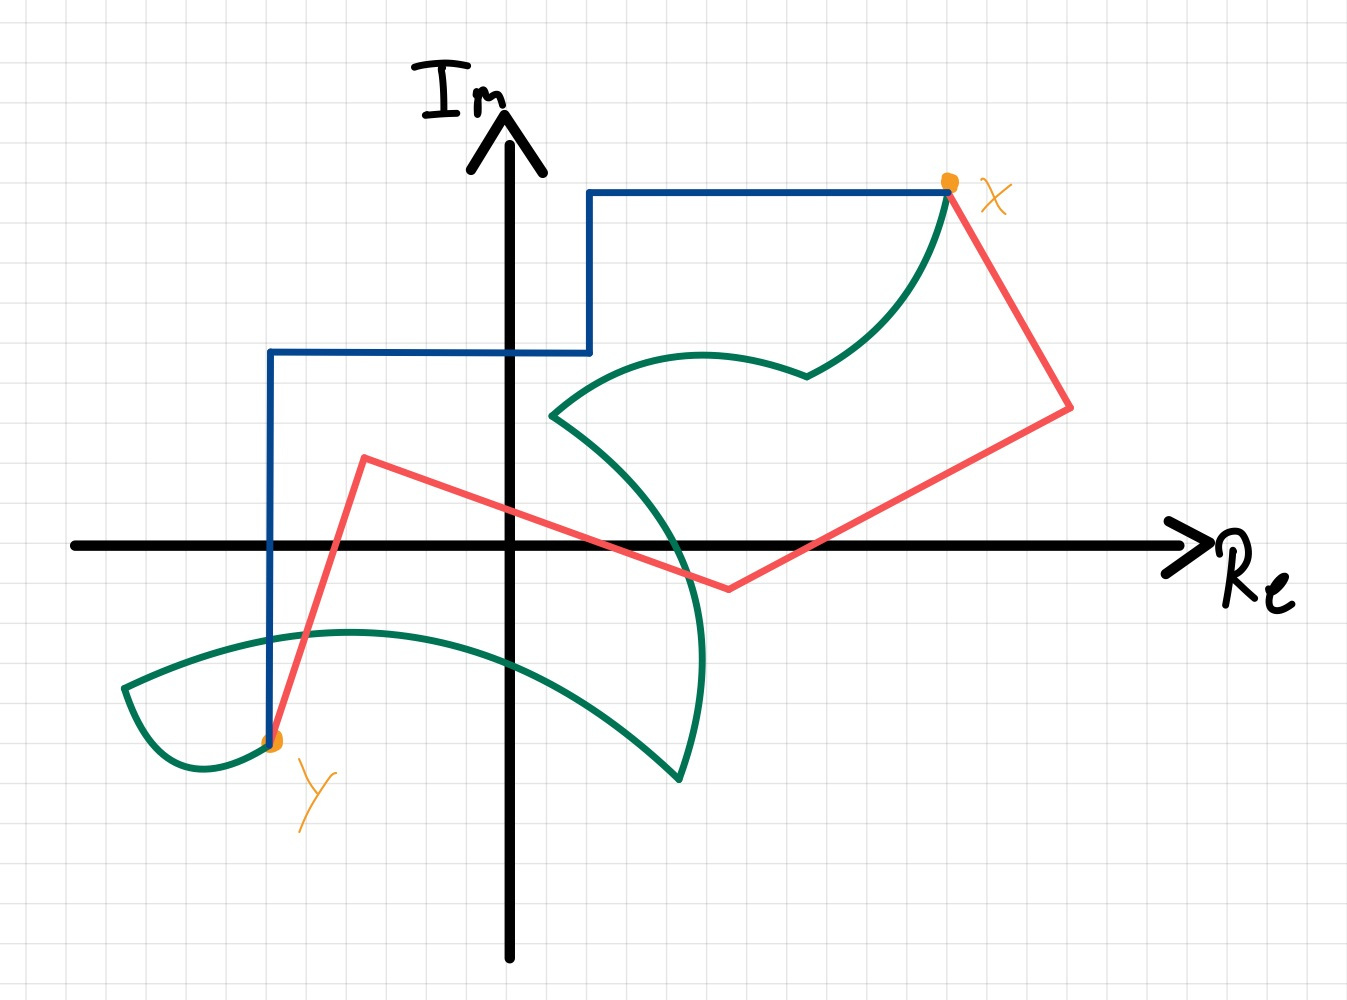
\includegraphics[width=\textwidth]{../\string_build/html/\string_images/treppenzug.jpg}
\caption{Visualisierung eines Integrationswegs in grün, eines Polygonzugs in rot und eines Treppenzugs in blau.}\label{\detokenize{complexanalysis/kurvenintegrale:fig-treppenzug}}\end{figure}

\par
Analog definiert man hier den Begriff des Integrals.
\begin{definition}{}{complexanalysis/kurvenintegrale:definition-7}



\par
Es sei \(U\subset\C\) eine offene Teilmenge und \(f:U\to\C\) eine stetige Funktion, für einen Integrationsweg \(\gamma:[a,b]\to\C\) mit Zerlegung \((t_0,\ldots,t_N)\)  definieren wir das \textbf{Wegintegral}
\begin{align*}
\int_\gamma f(z)\, dz:= \sum_{j=0}^{N-1} \int_{\gamma\rvert_{[t_j,t_{j+1}]}} f(z)\,dz.
\end{align*}\end{definition}
\begin{remark}{}{complexanalysis/kurvenintegrale:remark-8}



\par
Für einen Weg \(\gamma\) können verschiedene Zerlegungen \((t_0,\ldots,t_N)\) s.d., \(\gamma\) ein Integrationsweg bezüglich dieser Zerlegung ist. Man erkennt aber leicht, dass de Wert des Wegintegrals \textbf{unabhängig} von der Wahl der Zerlegung ist
\end{remark}

\par
Die Definition des Wegintegral ist unabhängig von Umparametrisierungen eines Weges, dies ist Inhalt des folgenden Lemmas.
\begin{lemma}{}{complexanalysis/kurvenintegrale:lemma-9}



\par
Es sei \(U\subset\C\) offen, \(\gamma:[a,b]\to U\) ein stetig differenzierbarer Weg und \(\phi:[c,d]\to[a,b]\) eine stetig differenzierbare Abbildung mit \(\phi(c)=a,\phi(d)=b\). Ist \(f:U\to\C\) stetig, so gilt
\begin{align*}
\int_{\gamma\circ\phi} f(z)\, dz = \int_\gamma f(z)\, dz.
\end{align*}\end{lemma}

\begin{proof}
 ToDo.
\end{proof}

\par
Insbesondere rechtfertigt diese Aussage, dass wir für den Strahl
\begin{align*}
[p,q]:=\{z\in\C: z = p+t(q-p), 0\leq t\leq 1\}
\end{align*}
\par
setzten
\begin{align*}
\int_{[p,q]} f(z)\, dz = \int_0^1 f(p+t(q-p))\cdot (q-p)\, dt.
\end{align*}

\subsection{Stammfunktionen}
\label{\detokenize{complexanalysis/kurvenintegrale:stammfunktionen}}
\par
Analog zum Begriff einer Stammfunktion in \(\R\) betrachten wir dieses Konzept nun für Funktionen \(f\C\to\C\).
\begin{definition}{}{complexanalysis/kurvenintegrale:definition-10}



\par
Es sei \(U\subset\C\) offen, eine holomorphe Funktion \(F:U\to\C\) heißt Stammfunktion einer Funktion \(f:U\to\C\), falls
\begin{align*}
F^\prime = f.
\end{align*}\end{definition}
\begin{remark}{}{complexanalysis/kurvenintegrale:remark-11}



\par
Wir beachten, dass in der obigen Definition die komplexe Ableitung benutzt wird.
\end{remark}

\par
Für reelle Funktionen schafft der Hauptsatz der Differentiations  und Integrationsrechnung (HDI) einen Zusammenhang zwischen dem Integral der Ableitung und der Stammfunktion. Mithilfe des Wegintegrals wollen wir nun ein ähnliches Konzept erarbeiten und bemerken zunächst folgende Tatsache.
\begin{lemma}{(Integral einer Ableitung)}{complexanalysis/kurvenintegrale:lem:intdiff}



\par
Es sei \(U\subset\C\) offen und \(f:U\to\C\) sei eine holomorphe Funktion, dann gilt
\begin{align*}
\int_\gamma f^\prime(z)\, dz= f(\gamma(b)) - f(\gamma(a))
\end{align*}
\par
für jeden Integrationsweg \(\gamma:[a,b]\to U\).
\end{lemma}

\begin{proof}
 Sei \(\gamma:[a,b]\to\C\) zunächst stetig differenzierbar, dann gilt
\begin{align*}
\int_\gamma f^\prime(z)\, dz = \int_a^b f^\prime(\gamma(t))\gamma^\prime(t)\, dt =(\#).
\end{align*}
\par
Die Abbildung \((f\circ \gamma):[a,b]\to\C\) ist reell differenzierbar und mit der Kettenregel auf \(\R\) gilt
\begin{align*}
(f\circ\gamma)^\prime = (f^\prime\circ\gamma)\cdot\gamma.
\end{align*}
\par
Daher folgt
\begin{align*}
(\#) = \int_a^b (f\circ \gamma)^\prime(t)\, dt.
\end{align*}
\par
Nach dem Hauptsatz der Integrations und Differentialrechnung für reelle Funktionen folgt dann
\begin{align*}
(\#) = f(\gamma(b)) - f(\gamma(a)).\end{align*}\end{proof}

\par
Anstatt allgemeiner offener Teilmengen \(U\subset\C\) zu betrachten schränkt man sich oft auf \textbf{Gebiete} ein.
\begin{definition}{}{complexanalysis/kurvenintegrale:definition-13}



\par
Eine offenen Menge \(U\subset\C\) heißt \textbf{Gebiet}, falls sie zusammenhängend ist, das heißt für zwei in \(U\) offene Mengen \(A,B\subset U,A\neq\emptyset\neq B\) gilt
\begin{align*}
A\cap B \neq \emptyset.
\end{align*}\end{definition}

\par
Für Gebiete gibt es folgende hilfreiche Charakterisierungen.
\begin{lemma}{}{complexanalysis/kurvenintegrale:lemma-14}



\par
Eine Menge \(U\subset\C\) ist genau dann ein Gebiet, falls eine der folgenden Bedingungen gilt.
\begin{enumerate}

\item {} 
\par
Die Menge \(U\) ist wegzusammenhängend, d.h., für \(x,y\in U\) existiert stets ein Weg \(\gamma:[a,b]\to U\) mit \(\gamma(a)=x,\gamma(b)=y\).

\item {} 
\par
Die Menge \(U\) ist polygonzusammenhängend, d.h., für \(x,y\in U\) existiert ein Polygonzug \(\gamma:[a,b]\to U\) mit \(\gamma(a)=x,\gamma(b)=y\).

\item {} 
\par
Die Menge \(U\) ist treppenzusammenhängend, d.h., für \(x,y\in U\) existiert ein Treppenzug \(\gamma:[a,b]\to U\) mit \(\gamma(a)=x,\gamma(b)=y\).

\end{enumerate}
\end{lemma}

\begin{proof}
 Siehe z.B. \cite{Nee17} Lemma 3.12.
\end{proof}

\par
Auf Gebieten können wir mithilfe von \cref{complexanalysis/kurvenintegrale:lem:intdiff} folgende Aussage zeigen.
\begin{lemma}{}{complexanalysis/kurvenintegrale:lemma-15}



\par
Es sei \(U\subset\C\) ein Gebiet, eine Funktion \(f:U\to\C\) ist genau dann konstant wenn \(f^\prime=0\) gilt.
\end{lemma}

\begin{proof}
 Falls \(f\) konstant ist folgt per Definition \(f^\prime=0\). Ist umgekehrt \(f^\prime=0\) dann finden wir für beliebige \(x,y\in U\) einen Polygonzug \(\gamma:[a,b]\to U, \gamma(a)=x,\gamma(b)=y\) mit Zerlegung \((t_0,\ldots,t_N)\), da \(U\) ein Gebiet ist. Dieser Weg ist insbesondere ein Inetgrationsweg und mit \cref{complexanalysis/kurvenintegrale:lem:intdiff} folgt dann
\begin{align*}
f(x) - f(y) = \int_\gamma f^\prime(z)\, dz = 0.
\end{align*}
\par
Da \(x,y\in U\) beliebig waren ist \(f\) konstant.
\end{proof}

\par
Im folgende formulieren wir ein zentrales Resultat für Stammfunktionen holomorpher Funktionen.
\begin{theorem}{(Existenz von Stammfunktionen)}{complexanalysis/kurvenintegrale:theorem-16}



\par
Es sei \(U\subset\C\) offen, dann besitzt eine stetige Funktion genau dann eine Stammfunktion, falls
\begin{align*}
\oint_\gamma f(z)\, dz =0
\end{align*}
\par
für jeden geschlossenen Integrationsweg \(\gamma\) gilt.

\par
Fixieren wir einen Punkt \(p\in\C\) und ist zusätzlich \(U\) zusammenhängend, so ist eine Stammfunktionen \(F:U\to\C, F(p)=c\in\C\) gegeben durch
\begin{align*}
F(w):= c+ \int_{\gamma_w} f(z) \,dz
\end{align*}
\par
wobei \(\gamma_w\) ein beliebiger Integrationsweg von \(p\) nach \(w\) ist.
\end{theorem}

\begin{proof}
 Siehe z.B. \cite{Nee17} Satz 3.17.
\end{proof}

\par
Die Bedingung an \(f\), dass alle Wegintegrale über geschlossene Wege wegfallen ist in der Praxis schwer nachzuprüfen. Für holomorphe Funktionen hat man allerdings folgendes praktische Korollar.
\label{complexanalysis/kurvenintegrale:corollary-17}
\begin{emphBox}{}{}{Corollary 7.1}



\par
Sei \(f:B_r(p)\to\C\) eine holomorphe Funktion auf der komplexen Scheibe \(B_r(p)\subset\C\) um \(p\) mit Radius \(r>0\), dann besitzt \(f\) eine Stammfunktion.
\end{emphBox}


\subsection{Integration über nicht differenzierbare Wege}
\label{\detokenize{complexanalysis/kurvenintegrale:integration-uber-nicht-differenzierbare-wege}}
\par
Mithilfe des Konzepts der Stammfunktion können wir nun das Integral über beliebige Wege definieren.
\begin{definition}{}{complexanalysis/kurvenintegrale:definition-18}



\par
Es sei \(\gamma:[a,b]\to U\) ein Weg, eine Zerlegung \((a=t_0,\ldots, t_N=b), t_j<t_{j+1}\) heißt \textbf{zulässig}, falls offenen Scheiben \(B^j\subset U\) existieren, s.d.
\begin{align*}
\gamma([t_j,t_{j+1}])\subset B^j\quad j=0,\ldots,N-1.
\end{align*}\end{definition}

\par
Für eine holomorphe Funktion \(f:U\to\C\) wissen wir dann, dass für einen Weg \(\gamma\) mit zulässiger Zerlegung \((t_0,\ldots,t_N)\) auf jeder Kreisscheibe \(B^j\subset U\) eine Stammfunktion \(F_j\) existiert, s.d.,
\begin{align*}
\int_\gamma f(z)\, dz= \sum_{j=0}^{N-1} \int_{\gamma\rvert_[t_j,t_{j+1}]} f(z)\, dz=
\sum_{j=0}^{N-1} F_j(\gamma(t_{j+1})) - F_j(\gamma(t_{j})).
\end{align*}
\par
Der Ausdruck auf der rechten Seite ist allerdings auch definiert, falls \(\gamma\) nicht differenzierbar ist, was auf folgende Definition führt.
\begin{definition}{}{complexanalysis/kurvenintegrale:definition-19}



\par
Es sei \(U\) offen und \(\gamma:[a,b]\to U\) ein Weg mit zulässiger Zerlegung \((t_0,\ldots,t_N)\) und offenen Kreisscheiben \(B_j,j=0,\ldots,N-1\). Für eine holomorphe Funktion \(f\) mit Stammfunktionen \(F_j\) auf \(B_j\) definieren wir
\begin{align*}
\int_\gamma f(z)\, dz = \sum_{j=1}^N F_j(\gamma(t_{j+1}))- F(\gamma(t_j)).
\end{align*}\end{definition}
\begin{remark}{}{complexanalysis/kurvenintegrale:remark-20}



\par
Für offenes \(U\subset\C\) und einen Weg \(\gamma:[a,b]\to U\) exsitiert stets eine zulässige Zerlegung und der Wert des Integrals ist unabhängig von der Wahl der Zerlegung, siehe \cite{Nee17}.
\end{remark}


\section{Der Integralsatz von Cauchy}
\label{\detokenize{complexanalysis/cauchyintegral:der-integralsatz-von-cauchy}}\label{\detokenize{complexanalysis/cauchyintegral::doc}}
\par
Wir wollen nun einen der zentralen Aussagen der Funktionentheorie formulieren, die Cauchysche Integralformel.
Diese besagt, dass sich die Werte einer holomorphen Funktion im Inneren eines bestimmten Gebietes bereits durch die Werte auf dem Gebietsrand bestimmen lassen. Ein erstes Resultat in diese Richtung erhalten wir indem wir \emph{benachbarte Wege} betrachten.


\subsection{Benachbarte Wege}
\label{\detokenize{complexanalysis/cauchyintegral:benachbarte-wege}}
\par
In der Definition eines Wegintegrals über beliebige Wege betrachtet man zulässige Zerlegungen mit offenen Kreisscheiben. Finden wir nun eine Zerlegung, s.d., sich zwei Wege die jeweiligen Kreisscheiben teilen, so wollen wir sie benachbart nennen.
\begin{definition}{}{complexanalysis/cauchyintegral:definition-0}



\par
Es sei \(U\subset \C\) offen und seien \(\gamma_0,\gamma_1:[a,b]\to U\) zwei Wege. Falls eine Zerlegung \((a=t_0,\ldots,b=t_N)\) existiert mit Kreisscheiben \(B^j\), welche zulässig für beide Wege ist, d.h.,
\begin{align*}
\gamma_0([t_j, t_{j+1}])\cup \gamma_1([t_j,t_{j+1}]) \subset B^j
\end{align*}
\par
dann nennen wir \(\gamma_0\) und \(\gamma_1\) \textbf{benachbart}.
\end{definition}

\par
Der Begriff der Nachbarschaft hat tatsächlich auch eine geometrische Bedeutung, welche in folgendem Lemma festgehalten wird.
\begin{lemma}{(Nachbarschaftslemma)}{complexanalysis/cauchyintegral:lem:closelem}



\par
Es sei \(U\subset\C\) offen, dann existiert ein \(\varepsilon>0\), s.d. falls für zwei Wege \(\gamma_0,\gamma_1:[a,b]\to U\) gilt
\begin{align*}
\abs{\gamma_0 - \gamma_1} < \varepsilon
\end{align*}
\par
so folgt schon, dass \(\gamma_0,\gamma_1\) benachbart sind.
\end{lemma}

\begin{proof}
 Siehe z.B. \cite{Nee17}.
\end{proof}

\par
Für benachbarte Wege erhalten wir nun das folgende Resultat, welches eine Vorstufe zum Integralsatz von Cauchy darstellt.
\begin{lemma}{}{complexanalysis/cauchyintegral:lem:closepath}



\par
Es \(U\subset\C\) eine offene Menge und \(f:U\to\C\) eine holomorphe Funktion, weiterhin seien \(\gamma_0,\gamma_1:[a,b]\to U\) zwei benachbarte Weg die eine der folgenden Bedingungen erfüllen
\begin{enumerate}

\item {} 
\par
die Wege haben gleiche Anfangs  und Endpunkte, oder

\item {} 
\par
die Wege sind geschlossen.

\end{enumerate}

\par
Dann gilt
\begin{align*}
\int_{\gamma_0} f(z)\, dz = \int_{\gamma_1} f(z)\, dz.
\end{align*}\end{lemma}

\begin{proof}
 Siehe z.B. {[}{]} Lemma 4.5.
\end{proof}


\subsection{Homotopie}
\label{\detokenize{complexanalysis/cauchyintegral:homotopie}}
\par
Um nicht nur benachbarte Wege betrachten zu können definieren wir jetzt den Begriff von Homotopie.
\begin{definition}{}{complexanalysis/cauchyintegral:definition-3}



\par
Es sei \(U\subset\C\) offen, zwei Wege \(\gamma_0, \gamma_1:[a,b]\to U\) mit gleichen Anfangs und Endpunkten,
\begin{align*}
\gamma_0(a) = \gamma_1(a),\\
\gamma_0(b) = \gamma_1(b),
\end{align*}
\par
heißen \textbf{homotop}, falls eine stetige Abbildung \(h:[a,b]\times[0,1]\to U\) existiert, so dass für alle \(t\in[a,b]\) gilt
\begin{align*}
h(t,0) = \gamma_0(t), \qquad h(t,1) = \gamma_1(t).
\end{align*}
\par
In diesem Fall nennen wir die Abbildung \(h\) eine \textbf{Homotopie} zwischen den Wegen \(\gamma_0\) und \(\gamma_1\) und notieren auch \(h_s:=h(\cdot,s):[a,b]\to U\) für den Weg am Punkt \(s\in [0,1]\).
\end{definition}

\par
Anstatt nur Wege mit gleichen Anfangs und Endpunkten zu betrachten können wir auch Homotopie geschlossener Wege definieren.
\begin{definition}{}{complexanalysis/cauchyintegral:definition-4}



\par
Es sei \(U\subset\C\) offen, zwei geschlossene Wege \(\gamma_0, \gamma_1:[a,b]\to U\) heißen \textbf{frei homotop}, falls eine stetige Abbildung \(h:[a,b]\times[0,1]\to U\) existiert, so dass für alle \(t\in[a,b]\) gilt
\begin{align*}
h(t,0) = \gamma_0(t), \qquad h(t,1) = \gamma_1(t)\quad
\end{align*}
\par
und der Weg \(h_s\) geschlossen ist für alle \(s\in [0,1]\).

\par
Ein geschlossener Weg heißt \textbf{zusammenziehbar} oder \textbf{nullhomotop}, falls er frei homotop zu einem konstanten Weg ist.
\end{definition}
\begin{remark}{}{complexanalysis/cauchyintegral:remark-5}



\par
Man kann zeigen, dass der Begriff der Homotopie zwischen Wegen in einer Teilmenge \(U \subset \C\) eine \emph{Äquivalenzrelation} auf Wegen in \(U\) induziert. Die zugehörigen Äquivalenzklassen werden auch \emph{Homotopieklassen} genannt.
\end{remark}


\subsection{Der Homotopiesatz und der Integralsatz von Cauchy}
\label{\detokenize{complexanalysis/cauchyintegral:der-homotopiesatz-und-der-integralsatz-von-cauchy}}
\par
Für geschlossene Wege impliziert Homotopie eine besondere Eigenschaft bezüglich des Kurvenintegrals, wie folgendes Lemma festhält.
\begin{lemma}{}{complexanalysis/cauchyintegral:lem:homotop}



\par
Es sei \(U \subset \C\) offen und seien \(\gamma_0\) und \(\gamma_1:[a,b]\to U\) homotope oder frei homotope Wege.
Sei außerdem \(f:U\to C\) eine holomorphe Funktion, dann gilt
\begin{align*}
\oint_{\gamma_0} f(z) \, dz = \oint_{\gamma_1} f(z) \, dz.
\end{align*}\end{lemma}

\begin{proof}
 Es sei \(h:[a,b]\times[0,1]\to U\) eine Homotopie, mit \(h_0=\gamma_0, h_1=\gamma_1\). Die Menge \([a,b]\times[0,1]\) ist kompakt und somit ist \(h\) gleichmäßig stetig, d.h. insbesondere, dass für \(\varepsilon>0\) ein \(\delta >0\) existiert, s.d.,
\begin{align*}
\abs{h_{s_0}-h_{s_1}}_\infty <\varepsilon \text{ für } \abs{s_1-s_2}< \delta.
\end{align*}
\par
Wir können nach \cref{complexanalysis/cauchyintegral:lem:closelem} somit \(\delta\) klein genug wählen, s.d. Wege \(h_{s_0}, h_{s_1}\) benachbart sind für \(\abs{s_0-s_1}<\delta\). Somit gilt nach \cref{complexanalysis/cauchyintegral:lem:closepath}  dass
\begin{align*}
\int_{h_{s_0}} f(z)\, dz = \int_{h_{s_1}} f(z)\, dz
\end{align*}
\par
gilt für \(\abs{s_0-s_1}<\delta\). Damit folgt die Aussage.
\end{proof}

\par
Es folgt, dass das Kurvenintegral einer holomorphe Funktionen über einen nullhomotopen Weg verschwindet, was als \textbf{Integralsatz von Cauchy} bekannt ist.
\begin{theorem}{(Integralsatz von Cauchy)}{complexanalysis/cauchyintegral:theorem-7}



\par
Es sei \(U\subset\C\) offen und sei \(\gamma:[a,b]\to U\) ein nullhomotoper Weg, für jede holomorphe Funktion \(f:U\to\C\) gilt dann
\begin{align*}
\oint_\gamma f(z)\, dz = 0.
\end{align*}\end{theorem}

\begin{proof}
 Folgt direkt aus \cref{complexanalysis/cauchyintegral:lem:homotop} 
\end{proof}


\subsection{Die Integralformel von Cauchy}
\label{\detokenize{complexanalysis/cauchyintegral:die-integralformel-von-cauchy}}
\par
Wir werden die obigen Konzepte nun auf Wegen betrachten welche den rnd einer Kreisscheibe parametrisieren. Dazu sei \(B_r(p)\subset\C\) eine Kreisscheibe um den Punkt \(p\in\C\) mit Radius \(r>0\), wir wählen die natürliche Parametrisierung des Randes
\begin{align*}
\gamma_{p,r}:[0,2\pi]&\to \partial B_r(p)\\
t&\mapsto p + r\exp(i t),
\end{align*}
\par
wobei wir die Eulersche Formel \eqref{equation:complexanalysis/complexnumbers:eq:euler} benutzt haben.

\par
Mithilfe der natürlichen Parametrisierung schreiben wir auch
\begin{align*}
\int_{\partial B_r(p)} f(z)\, dz := \int_{\gamma_{p,r}} f(z)\, dz
\end{align*}
\par
und formulieren nun die Integralformel von Cauchy.
\begin{theorem}{(Cauchy Integralformel)}{complexanalysis/cauchyintegral:theorem-8}



\par
Sei \(U \subset \C\) offen, \(\overline{B_r(p)}\subset \C\) und \(f:U\to \C\) holomorph\$, dann gilt
\begin{align*}
f(w) = \frac{1}{2\pi i} \int_{B_r(p)} \frac{f(z)}{z-w}\, dz
\end{align*}
\par
für alle \(w\in B_r(p)\).
\end{theorem}

\begin{proof}
 Siehe z.B. \cite{Nee17} Satz 4.13.
\end{proof}

\par
Als Korollar erhält man die Tatsache, dass Ableitungen holomorpher Funktionen selbst holomorph sind. Somit ist jede holomorphe Funktion unendlich oft differenzierbar.
\label{complexanalysis/cauchyintegral:cor:infholo}
\begin{emphBox}{}{}{Corollary 7.2}



\par
Es sei \(U\subset\C\) offen und \(f:U\to\C\) holomorph, dann ist \(f^\prime:U\to\C\) auch holomorph und für \(\overline{B_r(p)}\subset U\) gilt
\begin{align*}
f^{(n)}(w) = \frac{n!}{2\pi i} \int_{\partial B_r(p)} \frac{f(z)}{(z-w)^{n+1}}\, dz
\end{align*}
\par
für alle \(w\in B_r(p)\).
\end{emphBox}


\subsection{Der Satz von Liouville}
\label{\detokenize{complexanalysis/cauchyintegral:der-satz-von-liouville}}
\par
Eine weitere interessante Folgerung aus der Integralformel ist der Satz von Liouville.

\begin{emphBox}{Joseph Liouville}{}

\par
\href{https://de.wikipedia.org/wiki/Joseph\_Liouville}{Joseph Liouville} (Geboren 24. März 1809 in Saint Omer; Gestorben 8. September 1882 in Paris) war ein französischer Mathematiker.
\end{emphBox}
\begin{theorem}{(Satz von Liouville)}{complexanalysis/cauchyintegral:theorem-10}



\par
Jede beschränkte holomorphe Funktion \(f:\C\to\C\) ist konstant.
\end{theorem}

\begin{proof}
 Es gelte \(\abs{f(z)}< C <\infty\) für alle \(z\in\C\), dann gilt nach \cref{complexanalysis/cauchyintegral:cor:infholo}  dass
\begin{align*}
f^\prime(w) = \frac{1}{2\pi i} \int_{\partial B_r(w)} \frac{f(z)}{(z-w)^2}\, dz
\end{align*}
\par
für alle \(w\in \C\) und alle \(r> 0\). Damit folgt
\begin{align*}
\abs{f^\prime(w)}\leq \frac{C}{2 \pi} \abs{\int_{\partial B_r(w)} dz}\leq \frac{C}{r}.
\end{align*}
\par
Da diese Ungleichung für alle \(r>0\) und \(w\in\C\) gilt folgt \(\abs{f^\prime(w)} = 0\) für alle \(w\in\C\) und somit ist \(f\) konstant.
\end{proof}

\par
Hieraus folgt sofort der Fundamentalsatz der Algebra.
\begin{theorem}{(Fundamentalsatz der Algebra)}{complexanalysis/cauchyintegral:theorem-11}



\par
Hat ein Polynom
\begin{align*}
f(z)=\sum_{j=0}^N a_j z^j
\end{align*}
\par
keine Nullstellen, so ist es konstant.
\end{theorem}

\begin{proof}
 Wir nehmen o.B.d.A. an, dass \(a_N=1\) gilt. Dann existiert ein Polynom \(g\), s.d. \(f(z) = z^n + g(z)\) und
\begin{align*}
\lim_{z\to\infty} \frac{g(z)}{z^n} = 0,
\end{align*}
\par
wir finden also \(r>0\), s.d. \(\abs{g(z)} < 1/2 \abs{z^n}\) für alle \(\abs{z}>r\). Dann folgt auch
\begin{align*}
\abs{f(z)} = \abs{z^n + g(z)} \geq \abs{z^n} - 1/2 \abs{z^n}\geq r^n/2.
\end{align*}
\par
Besitzt \(f\) keine Nullstellen, so ist \(1/f:\C\to\C\) eine auf ganz \(\C\) holomorphe Funktion. Weiterhin gilt
\begin{align*}
\abs{1/f(z)} \leq \frac{2}{r^n}
\end{align*}
\par
für alle \(\abs{z}\geq r\) und somit
\begin{align*}
\abs{1/f} \leq \max\{\max_{B_r(0)} \abs{f(z)}, \frac{2}{r^n} \} < \infty
\end{align*}
\par
daher ist \(1/f\) beschränkt und nach dem Satz von Liouville konstant. Damit ist auch \(f\) konstant.
\end{proof}


\section{Potenzreihen}
\label{\detokenize{complexanalysis/powerseries:potenzreihen}}\label{\detokenize{complexanalysis/powerseries::doc}}
\par
In diesem Abschnitt wollen wir genauer auf analytische Funktionen bzw. Potenzreihen eingehen, wir betrachten also Funktionen
\begin{align*}
z\mapsto \sum_{j=0}^{\infty} a_j (z-p)^j,
\end{align*}
\par
mit komplexen Koeffizienten \(a_j\in\C\).


\subsection{Analytische Funktionen}
\label{\detokenize{complexanalysis/powerseries:analytische-funktionen}}
\par
Wir betrachten zunächst Funktionen welche durch Potenzreihen gegeben sind und erhalten, dass sie auf Kreisscheiben schon holomorph sind.
\begin{lemma}{}{complexanalysis/powerseries:lem:potseries}



\par
Es sei \(a_j\in\C, j\in\N_0\) eine Folge komplexer Zahlen, \(p\in\C\) und die Reihe
\begin{align*}
\sum_{j=0}^\infty a_j (z_0-p)^j\end{align*}
\par
konvergiere für \(z\neq p\). Dann ist die Funktion \(f:z\mapsto \sum_{j=0}^\infty a_j (z-p)^j\) holomorph auf der Kreisscheibe \(B_r(p)\), wobei \(r:=\abs{z_0-p}\) und
\begin{align*}
f^\prime(z) = \sum_{j=1}^\infty a_j\cdot j\cdot (z-p)^{j-1}.
\end{align*}\end{lemma}

\begin{proof}
 Siehe \cite{Nee17} Satz 2.19.
\end{proof}

\par
Eine besondere Klasse von Funktionen sind \emph{analytische Funktonen}, die sich lokal mit Hilfe von Reihen darstellen lassen.
\begin{definition}{}{complexanalysis/powerseries:definition-1}



\par
Sei \(U \subset \C\) offen und \(f: U\to \C\) eine Funktion.

\par
Wir nennen \(f\) \textbf{analytisch} in einem Punkt \(p \in U\) genau dann, wenn ein \(r > 0\) existiert, so dass sich die Funktion lokal in \(B_r(p)\) als Potenzreihe darstellen lässt,
\begin{align*}
f(z) = \sum_{j=0}^\infty a_j (z-p)^j, \qquad \forall z\in B_r(p)
\end{align*}
\par
wobei \((a_n)_{n_\in\N}\) eine Folge in \(\C\) ist.

\par
Wir nennen die Funktion \(f\) analytisch auf der Teilmenge \(U\), wenn sie analytisch ist für alle Punkte \(z_0 \in D\).
\end{definition}

\par
Der folgende Satz beschreibt den Zusammenhang zwischen analytischen und holomorphen Funktionen.
\begin{theorem}{}{complexanalysis/powerseries:thm:analytischHolomorph}



\par
Jede analytische Funktion \(f\) auf einer Teilmenge \(U \subset \C\) ist auch holomorph auf \(U\).
\end{theorem}

\begin{proof}
 Folgt direkt aus \cref{complexanalysis/powerseries:lem:potseries} \end{proof}

\par
Wir wollen im folgenden sehen, dass auch die Umkehrung gilt.


\subsection{Konvergenzradius}
\label{\detokenize{complexanalysis/powerseries:konvergenzradius}}
\par
Ein wichtige Eigenschaft von Potenzreihen um \(p\in\C\) ist, dass Konvergenz an einem Punkt \(z\) schon die absolute und gleichmäßige Konvergenz innerhalb einer Kreisscheibe impliziert.
\begin{lemma}{}{complexanalysis/powerseries:lem:powerradius}



\par
Konvergiert die Reihe \(\sum_{j=0}^\infty a_j (z_0-p)^j\) für \(z_0\in\C\), so konvergiert die Reihe \(\sum_{j=0}^\infty a_j (z-p)^n\) auf jeder offenen Kreisscheibe \(B_r(p)\) mit \(r< \abs{z_0 - p}\).
\end{lemma}

\begin{proof}
 O.B.d.A. gelte \(p=0\), da \(\sum_{j=0}^\infty a_j z_0^j\) konvergiert ist, \(a_j z_0^j\) eine Nullfolge und insbesondere existiert eine Konstante \(C>0\), s.d., \(\abs{a_j z_0^j}< C\) für alle \(j\in\N\). Sei nun \(r<\abs{z_0}\), dann folgt für jedes \(z\in B_r(0)\), dass
\begin{align*}
\abs{a_j z^j} = \abs{a_j z_0^j}\abs{\frac{z}{z_0}}^j\leq C \left(\frac{r}{z_0}\right)^j
\end{align*}
\par
und damit
\begin{align*}
\sum_{j=0}^\infty \abs{a_j z_j} \leq C \sum_{j=0}^\infty \left(\frac{r}{z_0}\right)^j
\end{align*}
\par
wobei die geometrische Reihe auf der linken Seite konvergiert. Somit konvergiert die Reihe auf \(B_r(0)\) nach dem Majorantenkriterium gleichmäßig absolut.
\end{proof}

\par
Der maximale Radius für welchen eine Potenzreihe konvergiert, wird als Konvergenzradius bezeichnet.
\begin{definition}{}{complexanalysis/powerseries:definition-4}



\par
Für eine Koeeffizientenfolge \(a_j\in\C\) und \(p\in\C\) ist der \textbf{Konvergenzradius} der Potenzreihe definiert durch
\begin{align*}
R :=\sup\left\{\abs{z - p}: \sum_{j=0}^\infty a_j (z-p)^j \text{ konvergiert}\right\}.
\end{align*}\end{definition}

\par
Die Definition ist äquivalent zum Wert
\begin{align*}
R :=\sup\left\{r<0: \sum_{j=0}^\infty a_j r^j\text{ konvergiert} \right\}
\end{align*}
\par
was auf das bekannte \textbf{Wurzelkriterium} führt.


\subsection{Entwicklungssatz}
\label{\detokenize{complexanalysis/powerseries:entwicklungssatz}}
\par
In diesem Abschnitt erarbeiten wir mithilfe von Potenzreihen die komplexe Taylorreihe.

\begin{emphBox}{Brook Taylor}{}

\par
\href{https://de.wikipedia.org/wiki/Brook\_Taylor}{Brook Taylor} (Geboren 18. August 1685 in Edmonton, Middlesex; Gestorben 29. Dezember 1731 in Somerset House, London) war ein britischer Mathematiker und Mitglied der Royal Society.
\end{emphBox}
\begin{theorem}{(Entwicklungssatz)}{complexanalysis/powerseries:theorem-5}



\par
Es sei \(B_r(p)\) eine offene Kreisscheibe um \(p\in\C\) und \(f:B_r(p)\to\C\) eine Funktion. Die Funktion \(f\) ist genau dann holomorph, wenn sie durch eine konvergente Potenzreihe mit Entwicklungspunkt \(p\) dargestellt werden kann, d.h. falls eine Folge \(a_j\in\C\) existiert, s.d.,
\begin{align*}
f(z) = \sum_{j=0}^\infty a_j (z-p)^n.
\end{align*}
\par
In diesem Fall gilt insbesondere
\begin{align*}
a_n = \frac{1}{n!} f^{(n)}(p)
\end{align*}\end{theorem}
\begin{remark}{}{complexanalysis/powerseries:remark-6}



\par
Diese Aussage bildet das Gegenstück zur Tatsache das analytische Funktionen holomorph sind. Insbesondere ist die Reihe die man so erhält die Taylorreihe
\begin{align*}
\sum_{j=0}^\infty \frac{1}{n!} f^{(n)}(p) (z-p)^n.
\end{align*}\end{remark}

\begin{proof}
 ToDo, siehe \cite{Nee17} Satz 5.7.
\end{proof}
\begin{example}{}{complexanalysis/powerseries:example-7}



\par
ToDo, sehr wichtiges Beispiel aus \cite{Nee17} 5.10.
\end{example}


\section{Laurententwicklung und Residuensatz}
\label{\detokenize{complexanalysis/residuensatz:laurententwicklung-und-residuensatz}}\label{\detokenize{complexanalysis/residuensatz::doc}}
\par
In diesem Abschnitt betrachten wir nun Singularitäten holomorpher Funktionen auf gelochten Kreisscheiben. Konkret betrachten wir holomorphe Funktionen \(f:B_r(p)\setminus\{p\}\to\C\) und interessieren uns speziell für das Verhalten nahes des entfernten Mittelpunktes \(p\in\C\).


\subsection{Singularitäten holomorpher Funktionen}
\label{\detokenize{complexanalysis/residuensatz:singularitaten-holomorpher-funktionen}}
\par
In diesem Abschnitt beschäftigen wir uns mit speziell ausgezeichneten Punkten, den sogenannten Singularitäten.
\begin{definition}{}{complexanalysis/residuensatz:definition-0}



\par
Sei \(U \subset \C\) offen und \(p\in U\) ein Punkt und \(f: U \setminus \{p\}\to\C\) eine holomorphe Funktion ist, dann nennen wir den Punkt \(p\) eine \textbf{isolierte Singularität} von \(f\).
\begin{enumerate}

\item {} 
\par
Der Punkt \(p\in U\) heißt \textbf{hebbare Singularität}, falls \(p\) eine isolierte Singularität ist und es eine holomorphe Funktion \(g:U\to\C\) gibt, so dass \(g(z) = f(z)\) gilt für alle \(z \in U \setminus \{p\}\).

\item {} 
\par
Der Punkt \(p\in U\) heißt \textbf{Pol}, wenn ein \(k\in\N\) existiert, s.d., \(z\mapsto (z-p)^k f(z)\) eine hebbare Singularität in \(p\) hat. Das kleinste \(k\in\N\), das diese erfüllt heißt \textbf{Ordnung} des Pols.

\item {} 
\par
Wir nennen den Punkt \(p\) eine \textbf{wesentliche Singularität}, wenn \(p\) weder hebbar noch Pol ist.

\end{enumerate}
\end{definition}

\par
Intuitiv ist eine Polstelle hebbar, falls die Funktion um die Polstelle herum beschränkt ist. Dies ist die Aussage des Riemannschen Hebbarkeitssatzes.
\begin{theorem}{}{complexanalysis/residuensatz:thm:hebbar}



\par
Es sei \(U\subset \C\) offen, \(p\in U\) und \(f:U\setminus\{p\}\to\C\) holomorph. Falls eine Umgebung \(V\subset U, p\in V\) existiert, s.d., \(f\) auf \(V\setminus\{p\}\) beschränkt ist, so ist \(p\) eine hebbare Singularität.
\end{theorem}

\begin{proof}
 Wir nehmen o.B.d.A. an, dass \(p=0\) gilt und betrachten die Funktion
\begin{align*}
g(z) :=
\begin{cases}
z^2\cdot f(z)&\text{ für } z\neq 0,\\
0&\text{ für } z=0.
\end{cases}
\end{align*}
\par
Dann gilt
\begin{align*}
\lim_{z\to 0} \frac{g(z) - g(0)}{z} = \lim_{z\to 0} z\cdot f(z) =0
\end{align*}
\par
da \(f\) beschränkt in einer Umgebung um \(0\) ist. Somit ist \(g\) holomorph auf \(U\) und lässt sich damit als Potenzreihe in der \(0\) entwickeln,
\begin{align*}
g(z) = \sum_{j=0}^\infty a_j z^j,\quad 0 = g(0) = a_0, 0=g^\prime(0)=a_1.
\end{align*}
\par
Insbesondere gilt dann für \(z\in U\setminus\{0\}\)
\begin{align*}
f(z) = g(z)/z^2 = \sum_{j=2}^\infty a_j z^{j-2}
\end{align*}
\par
wobei die Reihe auf der rechten Seite eine holomorphe Funktion auf ganz \(U\) definiert, daher ist \(0\) eine hebbare Singularität.
\end{proof}


\subsection{Laurent Reihen}
\label{\detokenize{complexanalysis/residuensatz:laurent-reihen}}
\par
Zusätzlich zu Potenzreihen betrachtet man für Singularitäten sogenannte \textbf{Laurent Reihen}, wobei man nicht nur Potenzen \((z-p)^j\) für \(j\in \N\) betrachtet, sondern auch negative Exponenten zulässt und somit effektive rationale Funktionen \(\frac{1}{(z-p)^j}\) hinzuaddiert.

\begin{emphBox}{Pierre Alphonse Laurent}{}

\par
\href{https://de.wikipedia.org/wiki/Pierre\_Alphonse\_Laurent}{Pierre Alphonse Laurent} (Geboren 18. Juli 1813 in Paris; Gestorben 2. September 1854 ebenda) war ein französischer Mathematiker.
\end{emphBox}
\begin{definition}{}{complexanalysis/residuensatz:definition-2}



\par
Für eine Folge \(a_j\in\C, j\in \Z\) nennen wir die Reihe
\begin{align*}
\sum_{j=-\infty}^\infty a_j (z-p)^j
\end{align*}
\par
\textbf{Laurent Reihe} am Entwicklungspunkt \(p\in\C\). Wir nennen die Reihe konvergent, falls die Teilsummen
\begin{align*}
\sum_{j=0}^\infty a_j (z-p)^j\qquad \sum_{j=1}^\infty a_{-j} \frac{1}{(z-p)^j}
\end{align*}
\par
konvergieren und setzten den Grenzwert als Summe der beiden einzelnen Grenzwerte.
\end{definition}

\par
Für Laurent Reihen erhält man zwei Konvergenzradien, jeweils für die beiden Teilsummen.
\begin{definition}{}{complexanalysis/residuensatz:definition-3}



\par
Für eine Laurent Reihe sei \(R>0\) der Konvergenzradius der Reihe
\begin{align*}
\sum_{j=0}^\infty a_j (z-p)^j
\end{align*}
\par
und \(\tilde{r}\) der Konvergenzradius der Reihe
\begin{align*}
\sum_{j=1}^\infty a_{-j} \frac{1}{(z-p)^j}.
\end{align*}
\par
Dann heißt \(R\) \textbf{äußerer} und \(\frac{1}{\tilde{r}}\) \textbf{innerer} Konvergenzradius.
\end{definition}

\par
Anstatt von Kreisscheiben betrachten wir hier nun offene Ringe
\begin{align*}
B_{r,R}(p) := \{z\in \C: r< \abs{z-p} < R\}
\end{align*}
\par
und erhalten folgende Aussage.
\begin{lemma}{}{complexanalysis/residuensatz:lemma-4}



\par
Es sei \(\sum_{j=-\infty}^\infty a_j (z-p)^j\) eine Laurent Reihe mit äußerem Konvergenzradius \(R\) und innerem Konvergenzradius \(r\), dann gilt
\begin{itemize}
\item {} 
\par
Die Reihe divergiert auf \$\textbackslash{}C\textbackslash{}setminus\textbackslash{}overline\{B\_\{r,R\}(p)\},

\item {} 
\par
Die Reihe konvergiert auf \(B_{r,R}(p)\),

\item {} 
\par
für \(r<\tilde{r}<\tilde{R}< R\) konvergiert die Reihe gleichmäßig absolut auf \(B_{\tilde{r},\tilde{R}}(p)\)

\end{itemize}
\end{lemma}

\begin{proof}
 Folgt direkt aus \cref{complexanalysis/powerseries:lem:powerradius} \end{proof}

\par
Analog zur Entwicklung in die Taylorreihe haben wir auf offenen Ringen eine Entwicklung in Laurent Reihen.
\begin{lemma}{}{complexanalysis/residuensatz:lem:laurent}



\par
Es sei \(f:B_{r,R}(p)\to\C\) holomorph, dann gilt
\begin{align*}
f(z) = \sum_{j=-\infty}^\infty a_j (z-p)^j,
\end{align*}
\par
wobei die Koeffizienten für \(j\in\Z\) gegeben sind durch
\begin{align*}
a_j = \frac{1}{2\pi i} \oint_{\partial B_s(p)} \frac{f(z)}{(z-p)^{j+1}} dz \text{ für beliebiges } s\in (r,R).
\end{align*}\end{lemma}

\begin{proof}
 ToDo, siehe \cite{Nee17} Satz 6.7.
\end{proof}

\par
Mithilfe der Laurent Entwicklung auf der gelochten Kreisscheibe \(B_{0,R}(p)\) können wir nun Singularitäten von holomorphen Funktionen charakterisieren.
\begin{lemma}{}{complexanalysis/residuensatz:lemma-6}



\par
Es sei \(f:U\setminus\{p\}\to\C\) holomorph, \(B_{0,R}(p)\subset U\setminus\{p\}\) und \(a_j\in\C, j\in\Z\) seien die Koeffizienten der Laurent Entwicklung auf \(B_{0,R}\) welche nach \cref{complexanalysis/residuensatz:lem:laurent} existieren. Dann gilt:
\begin{enumerate}

\item {} 
\par
Die Singularität \(p\) ist genau dann hebbar, wenn \(a_{j}=0\) für alle \(j<0\).

\item {} 
\par
Die Singularität \(p\) ist genau dann ein Pol der Ordnung \(k\in\N\), \(a_{-k}\neq 0\) und \(a_j = 0\) für alle \(j<k\).

\item {} 
\par
Die Singularität \(p\) ist genau dann wesentlich, falls \(a_{-j}\neq 0\) für fast alle \(j\in\N\).

\end{enumerate}
\end{lemma}

\begin{proof}
 \textbf{Ad 1.}

\par
Gilt \(a_j=0\) für alle \(j<0\) so ist die Laurent Reihe
\begin{align*}
f(z) = \sum_{0}^\infty a_j (z-p)^j,
\end{align*}
\par
holomorph von \(B_{0,R}(p)\) auf \(B_R(p)\) fortsetzbar und die Singularität somit hebbar.

\par
\textbf{Ad 2.}

\par
ToDo

\par
\textbf{Ad 3.}

\par
ToDo
\end{proof}
\begin{definition}{}{complexanalysis/residuensatz:definition-7}



\par
Sei \(D \subset \C\) eine offene Teilmenge.
Wir nennen eine Funktion \(f \colon D \rightarrow \C\) \textbf{meromorph} auf \(D\) genau dann, wenn eine lokalendliche Menge \(P\) existiert, so dass die Funktion \(f\) holomorph auf \(D \setminus P\) mit Polen in \(P\) ist.
\end{definition}
\begin{example}{(Meromorphe Funktionen)}{complexanalysis/residuensatz:example-8}



\par
Rationale Funktionen oder konkretes Beispiel

\par
Schulz Baldes S.332
\end{example}


\subsection{Der Satz von Casorati–Weierstraß}
\label{\detokenize{complexanalysis/residuensatz:der-satz-von-casorati-weierstrasz}}
\par
Für wesentliche Singularitäten \(p\) können wir weder einen Wert der Funktion am Punkt \(p\) definieren, noch feststellen, dass die Funktion hier eindeutig gegen unendlich strebt. Tatsächlich nimmt eine Funktion um eine wesentliche Singularität herum überaschend viele verschiedene Werte an. Diese ist die Aussage des Satzes von Casorati–Weierstraß.

\begin{emphBox}{Felice Casorati}{}

\par
\href{https://de.wikipedia.org/wiki/Felice\_Casorati\_(Mathematiker)}{Felice Casorati} (Geboren 17. Dezember 1835 in Pavia; Gestorben 11. September 1890 in Casteggio) war ein italienischer Mathematiker.
\end{emphBox}

\begin{emphBox}{Karl Weierstraß}{}

\par
\href{https://de.wikipedia.org/wiki/Karl\_Weierstra\%C3\%9F}{Karl Theodor Wilhelm Weierstraß} (Geboren 31. Oktober 1815 in Ostenfelde bei Ennigerloh, Münsterland; Gestorben 19. Februar 1897 in Berlin) war ein deutscher Mathematiker.
\end{emphBox}
\begin{theorem}{}{complexanalysis/residuensatz:theorem-9}



\par
Es sei \(U \subset \C\) offen und \(p\in U\) eine wesentliche Singularität der holomorphen Funktion \(f:U\setminus\{p\}\to\C\), dann gilt, dass \(f(U\setminus\{p\})\) dicht in \(\C\) liegt.
\end{theorem}

\begin{proof}
 Angenommen \(f(U\setminus\{p\})\) wäre nicht dicht, dann existiert ein \(w\in\C\) und ein \(r>0\), s.d.
\begin{align*}
B_r(w) \cap f(U\setminus\{p\}) = \emptyset.
\end{align*}
\par
Da das Bild von \(f\) somit einen echten Abstand zum Punkt \(p\) hat ist die Funktion
\begin{align*}
z\mapsto\frac{1}{f(z) - w}
\end{align*}
\par
beschränkt und holomorph auf \(U\setminus\{p\}\). Somit folgt mit dem Hebbarkeitssatz \cref{complexanalysis/residuensatz:thm:hebbar}  dass diese Funktion einen hebbaren Pol bei \(p\) hat und somit zur holomorphen Funktion \(h:U\to\C\) fortsetzbar auf \(U\) ist. Diese Funktion hat keine Nullstellen

\par
ToDo
\end{proof}


\subsection{Umlaufzahlen}
\label{\detokenize{complexanalysis/residuensatz:umlaufzahlen}}
\par
Wir definieren als Nächstes eine charakteristische Größe von geschlossenen Wegen in \(\C\), den sogenannten Index.
\begin{definition}{}{complexanalysis/residuensatz:definition-10}



\par
Sei \(\gamma \colon [0,1] \rightarrow \C\) ein geschlossener Weg in \(\C\) und \(w \in \C \setminus \operatorname{Bild}(\gamma)\) ein beliebiger Punkt außerhalb der zugehörigen Kurve von \(\gamma\).
Wir bezeichnen als \textbf{Index} von \(w\) bezüglich des Wegs \(\gamma\) folgende charakteristische Größe
\begin{align*}
\operatorname{Ind}_\gamma(w) \ := \ \oint_\gamma \frac{1}{z - w} \frac{\mathrm{d}z}{2\pi i} \ = \ \int_0^1 \frac{\gamma'(t)}{\gamma(t - w)} \frac{\mathrm{d}z}{2\pi i} \in \mathbb{Z}.
\end{align*}
\par
Häufig wird der Index auch \textbf{Windungszahl} von \(\gamma\) um \(w\) genannt.
Sie ist eine \emph{topologische Invariante}, die anschaulich beschreibt, wie häufig sich die zugehörige Kurve um den Punkt \(w\) windet.
\end{definition}

\par
\textbf{ToDo: Abbildung mit Beispiel von \href{https://de.wikipedia.org/wiki/Umlaufzahl\_(Mathematik)}{Wikipedia}}
\begin{lemma}{}{complexanalysis/residuensatz:lemma-11}



\par
Sei \(\gamma \colon [0,1] \rightarrow \C\) ein geschlossener Weg in \(\C\).
Dann ist die Abbildung, die jedem Punkt \(w \in \C \setminus \operatorname{Bild}(\gamma)\) außerhalb der zugehörigen Kurve seinen Index \(\operatorname{Ind_\gamma}(w)\) konstant auf jeder Zusammenhangskomponente bezüglich der Kurve von \(\gamma\).
\end{lemma}

\begin{proof}
 Schulz Baldes S.318f.
\end{proof}


\subsection{Cauchyscher Residuensatz}
\label{\detokenize{complexanalysis/residuensatz:cauchyscher-residuensatz}}
\par
Das folgende Lemma erlaubt die explizite Berechnung des Residuums.
\begin{lemma}{}{complexanalysis/residuensatz:lemma-12}



\par
Sei \(D \subset \C\) eine offene Teilmenge und \(z_0 \in D\) Pol einer holomorphen Funktion \(f \colon D \setminus \{z_0\} \rightarrow \C\).

\par
Für genügend kleine \(\epsilon > 0\) lässt sich das Residuum von \(f\) bei \(z_0\) angeben als
\begin{align*}
\operatorname{Res}_{z_0}(f) = \oint_{\partial B_\epsilon(z_0)} f(z) \frac{\mathrm{d}z}{2\pi i}.
\end{align*}
\par
Falls der Pol von Ordnung \(-m\) ist, lässt sich das Residuum von \(f\) bei \(z_0\) sogar angeben als
\begin{align*}
\operatorname{Res}_{z_0}(f) = \partial_z^{m-1}\left( (z-z_0)^m \frac{f(z)}{(m-1)!}\right)|_{z=z_0}.
\end{align*}\end{lemma}

\begin{proof}
 Schulz Baldes S.333f.
\end{proof}
\begin{example}{(Berechnung des Residuums)}{complexanalysis/residuensatz:example-13}



\par
Rationale Funktion bei Schulz Baldes S.335
\end{example}

\par
Der folgende Residuensatz von Cauchy stellt eine zentrale Aussage der Funktionentheorie vor.
\begin{theorem}{}{complexanalysis/residuensatz:theorem-14}



\par
Sei \(D \subset \C\) eine offene Teilmenge und \(f \colon D \rightarrow \C\) eine meromorphe Funktion mit endlicher Menge \(P \subset D\) von Polstellen.
Sei außerdem \(\gamma\) ein geschlossener und zusammenziehbarer Weg in \(D\) mit \(\operatorname{Bild}(\gamma) \cap P = \emptyset\).

\par
Dann gilt der folgende Zusammenhang
\begin{align*}
\int_\gamma f(z) \frac{\mathrm{d}z}{2\pi i} = \sum_{z_0 \in P} \operatorname{Ind}_\gamma(z_0) \operatorname{Res}_{z_0}(f).
\end{align*}\end{theorem}

\begin{proof}
 Schulz Baldes S.337
\end{proof}
\begin{remark}{}{complexanalysis/residuensatz:remark-15}



\par
Für holomorphe Funktionen \(f\) entspricht der Residuensatz gerade dem Cauchyschen Integralsatz.
Wenn \(D\) als Sterngebiet angenommen wird ist die Zusammenziehbarkeit des Wegs \(\gamma\) immer erfüllt.
\end{remark}
\begin{example}{}{complexanalysis/residuensatz:example-16}



\par
Viele konkrete Beispiele in Schulz Baldes S.338 344
\end{example}


